%%%%%%%%%%%%%%%%%%%%%%%%%%%%%%%%%%%%%%%%%
% Short Sectioned Assignment
% LaTeX Template
% Version 1.0 (5/5/12)
%
% This template has been downloaded from:
% http://www.LaTeXTemplates.com
%
% Original author:
% Frits Wenneker (http://www.howtotex.com)
%
% License:
% CC BY-NC-SA 3.0 (http://creativecommons.org/licenses/by-nc-sa/3.0/)
%
%%%%%%%%%%%%%%%%%%%%%%%%%%%%%%%%%%%%%%%%%
%----------------------------------------------------------------------------------------
%	PACKAGES AND OTHER DOCUMENT CONFIGURATIONS
%----------------------------------------------------------------------------------------
\documentclass[paper=a4, fontsize=12pt, liststotoc,bibtotoc]{scrartcl} % A4 paper and 11pt font size
\usepackage[utf8]{inputenc}
\usepackage[T1]{fontenc} % Use 8-bit encoding that has 256 glyphs
\usepackage{fourier} % Use the Adobe Utopia font for the document - comment this line to return to the LaTeX default
\usepackage[german]{babel} % English language/hyphenation
\usepackage{amsmath,amsfonts,amsthm} % Math packages
\usepackage{color}
\definecolor{darkblue}{rgb}{0,0,.5}
\usepackage[colorlinks,linkcolor=darkblue,citecolor=red,urlcolor=blue]{hyperref}

\usepackage{sectsty} % Allows customizing section commands
\allsectionsfont{\centering \normalfont\scshape} % Make all sections centered, the default font and small caps

\usepackage{fancyhdr} % Custom headers and footers
\pagestyle{fancyplain} % Makes all pages in the document conform to the custom headers and footers
%\fancyhead{T} % No page header - if you want one, create it in the same way as the footers below
\fancyhead[L]{Drohnen - unbemannte Flugobjekte}
\fancyhead[C]{}
\fancyhead[R]{Hausarbeit}
\fancyfoot[L]{} % Empty left footer
\fancyfoot[C]{Codewort: Findus} % Empty center footer
\fancyfoot[R]{\thepage} % Page numbering for right footer
\renewcommand{\headrulewidth}{1pt} % Remove header underlines
\renewcommand{\footrulewidth}{1pt} % Remove footer underlines
\setlength{\headheight}{13.6pt} % Customize the height of the header
\setlength{\footheight}{8mm}
\numberwithin{equation}{section} % Number equations within sections (i.e. 1.1, 1.2, 2.1, 2.2 instead of 1, 2, 3, 4)
\numberwithin{figure}{section} % Number figures within sections (i.e. 1.1, 1.2, 2.1, 2.2 instead of 1, 2, 3, 4)
\numberwithin{table}{section} % Number tables within sections (i.e. 1.1, 1.2, 2.1, 2.2 instead of 1, 2, 3, 4)
\setlength\parindent{0pt} % Removes all indentation from paragraphs - comment this line for an assignment with lots of text


\newcommand{\horrule}[1]{\rule{\linewidth}{#1}} % Create horizontal rule command with 1 argument of height

\author{Jan Sutmöller} % Your name

\date{\normalsize\today} % Today's date or a custom date
\bibliographystyle{unsrt}

%%%%%%%%%%%eigene Sachen%%%%%%%
\flushbottom 
\usepackage{graphicx}
\usepackage{microtype}    
% Abkürzungsverzeichniss
\usepackage[printonlyused]{acronym}
\usepackage{wrapfig}
% Inhaltsverzeichnis auch in Time New Roman
\addtokomafont{sectioning}{\rmfamily}
\usepackage[section]{placeins}

\pagestyle{empty}

%%%%%%%%%%%%%%%%%%%%%%%%%%%%%%%%%%%%%%%%%%%%%%%%%%%%%%%%%%
%%%%%%%%%%%%%%%%%%%%%%%%%%%%%%%%%%%%%%%%%%%%%%%%%%%%%%%%%%
%%%%%%%%%	Begin des eigentlichen Dokuments  %%%%%%%%%%%%
%%%%%%%%%%%%%%%%%%%%%%%%%%%%%%%%%%%%%%%%%%%%%%%%%%%%%%%%%%
%%%%%%%%%%%%%%%%%%%%%%%%%%%%%%%%%%%%%%%%%%%%%%%%%%%%%%%%%%


\begin{document}


%\maketitle % Print the title
\begin{center}
\begin{tabular}{p{\textwidth}}


\begin{center}
\includegraphics[scale=0.5]{img/HFTL-Logo.pdf}
\end{center}


\\

\begin{center}
\LARGE{\textsc{
Entwicklung einer HFTL-APP \\
Dokumentation\\
}}
\end{center}

\\


\begin{center}
\large{Studienmodul \textit{Software-Engineering} \\
der Hochschule für Telekommunikation\\
Leipzig\\}
\end{center}

\\

\begin{center}
\textbf{\Large{Projektarbeit - Softwareentwicklung}}
\end{center}


%\begin{center}
%zur Erlangung des akademischen Grades\\
%Bachelor of Engineering
%\end{center}


\begin{center}
vorgelegt von
\end{center}

\begin{center}
\large{\textbf{BKMI Matrikel 13}} \\
\small{}
\end{center}

\begin{center}
\large{23.04.2015}
\end{center}

\\

\\

\begin{center}
\begin{tabular}{lll}
\textbf{Dozent:} & & Profn. Dr.-Ing. Sabine Wieland\\
%\textbf{Zweitprüfer:} & &Prof. Dr.-Ing. F. Musterfrau\\
\end{tabular}
\end{center}

\end{tabular}
\end{center}
%\part im Inhaltsverzeichnis nicht nummerieren
\makeatletter
\let\partbackup\l@part
\renewcommand*\l@part[2]{\partbackup{#1}{}}

\newpage

%Seitennummerierung neu beginnen, Zahlen [arabic], röm.Zahlen [roman,Roman], Buchstaben [alph,Alph]
\pagenumbering{arabic}

\cleardoublepage\pdfbookmark{Inhaltsverzeichniss}{toc}

\tableofcontents
\listoffigures
\pagestyle{fancy}
\newpage

\section{Einleitung}

Der Begriff der Drohne begegnet uns in Deutschland überall im Alltag: In den Medien, Bekannte kaufen sich fast vollkommen autark fliegende Flugmaschinen. An Drohnen montierte, hochauflösende Kameras schießen Bilder, wie sie sonst nur von Fotografen aus Propellermaschinen gemacht werden konnten oder von Satelliten mit Millionen teurem Equipment \cite{holzapfel}. Weltweit herrschen große Diskussionen. Befürworter wie auch Kritiker stehen sich mit nachvollziehbaren Argumenten gegenüber. Es zieht sich ein schmaler Grat zwischen Nutzen und Problemen durch die Thematik. In Deutschland herrscht eine politisch gesetzliche Debatte über den neu aufkommenden Hype um die \glqq private\grqq\ Drohnen (\ac{UAV})\cite{welchedrohne}. 

In dieser Hausarbeit wird zunächst eine terminologische Begriffsbestimmung gemacht und dann auf die Geschichte eingegangen. Daraufhin wird konkretisierend auf die \glqq private\grqq\ Drohne DJI Phantom 2 Vision Plus eingegangen. Zum Schluss wird die rechtliche Situation in Deutschland in Bezug auf  \glqq private\grqq\ Drohnen erläutert.


\section{Begriffsklärung}
Das Wort \glqq Drohne\grqq\ ist eng mit dem militärischen Einsatz von unbemannten Flugkörpern verknüpft und wird mit dem Einsatz als tötende Waffe assoziiert. Es besteht keine Verknüpfung zu der Beschreibung eines unbewaffneten, vorwiegend für Freizeitaktivitäten und zivilen Einsatz eingesetzten Fluggerätes\cite{Buch_Engl}.


\ac{UAV} sind unbemannte Fluggeräte, welche entweder von Bodenpersonal gesteuert werden oder vollkommen autark fliegen. Es gibt sie in den verschiedensten Ausführungen, von einigen Zentimetern Größe(Revell Nano Quad) bis hin zu der Größe eines Jumbojets(Boeing Condor). Es gibt autark fliegende Hubschrauber, Flugzeuge und mehrrotorige \ac{UAV}. Selbst die von Wernher von Braun entwickelte \ac{V2} wird als ein selbständig fliegendes Objekt bezeichnet. Sie war  mit Mechanismen ausgestattet, die eine korrekte Zielführung sicherstellten und zur Not den Kurs automatisch anpassen konnten \cite{V2}.

\section{Allgemeines zu \acs{UAV}}
\subsection{Geschichte}

1849 gab es erste Aufzeichnungen von \ac{UAV}. Es waren mit Bomben bestückte Heißluftballons von österreichischen Entwicklern. Die Ballons wurden über einen Kupferdraht ferngezündet (Siehe Abbildung:   \ref{ballonbombs}). Charles Perley entwickelte dieses Verfahren im Jahre 1863 weiter, indem er Bomben per Zeitzünder abwarf \cite{baloonbombs}.

Im ersten Weltkrieg wurde von Elmer Sperry und Peter Cooper Hewitt das  Hewitt-Sperry Automatic Airplane (genannt: Flying Bomb, siehe Abbildung: \ref{Flying Bomb}) entwickelt. Dieses Flugzeug war in der Lage einen vordefinierten Kurs zu halten.
Zu einem bestimmten Zeitpunkt wurden geladene Torpedos ausgelöst. Sie konnten durch gyroskopische Stabilisierer die Richtung halten.\cite{flyingbomb}

In den 30iger Jahren entwickelte Reginald Denny funkgesteuerte Flugzeuge zum Training der US Army. 1935 entwarf er seine \ac{RP-1}, die er in den folgenden Jahren bis zur RP-5 weiterentwickelte. Die \ac{RP-1} war dafür ausgelegt, die Luftabwehrschützen der US Army zu trainieren, indem die \ac{RP-1} als Zielscheibe genutzt wurde. Sie war das erste, in Masse gefertigte, \ac{UAV}.\cite{RP-1}

1941 wurde in das \ac{UAV} namens \textit{Culver Cadet} eine Kamera eingebaut, die auf einem Bildschirm eines zweiten bemannten Flugzeuges zu sehen war, wodurch Einsätze einen viel größeren Radius haben konnten.

In den 60er Jahren rückte das Thema \emph{Überwachung von anderen Staaten} zunehmend in die Interessen der amerikanischen Verteidigungspolitik. Es wurde ein Langstreckenaufklärer vom Typ Ryan Model 147A (Codename: Fire Fly, siehe Abbildung \ref{fire fly}) entwickelt. Dieser konnte über Entfernungen von bis zu 1930 Kilometern operieren. Sie wurde eingesetzt um Länder wie Vietnam, Kuba, China und Nordkorea auszuspionieren.\cite{FireFly}

Der derzeitige Stand der Technik wird bei den Militär- \ac{UAV} durch die Northrop Grumman RQ-4(Global Hawk) definiert. Es kann in großen Höhen (bis zu 20 km) operieren. Die Flugzeit wird mit über 34 Std. angegeben(siehe Abbildung:\ref{global hawk}) \cite{rq-4}.


\subsection{Einsatzgebiete}
Es gibt die verschiedensten Einsatzgebiete unbemannter Luftfahrzeuge. Zum Einen gibt es den militärischen Sektor, indem \acp{UAV} dafür eingesetzt werden, um Aufklärungsflüge in extremen Höhen und großen Reichweiten zu ermöglichen. Die Northrop Grumman RQ-4 (Global Hawk)(siehe Abbildung:\ref{global hawk}) agiert zum Beispiel in einer Höhe von bis zu 20 Kilometer und hat einen Einsatzradius von 7500 Kilometern.

\begin{wrapfigure}{r}{0.5\textwidth}
  \begin{center}
    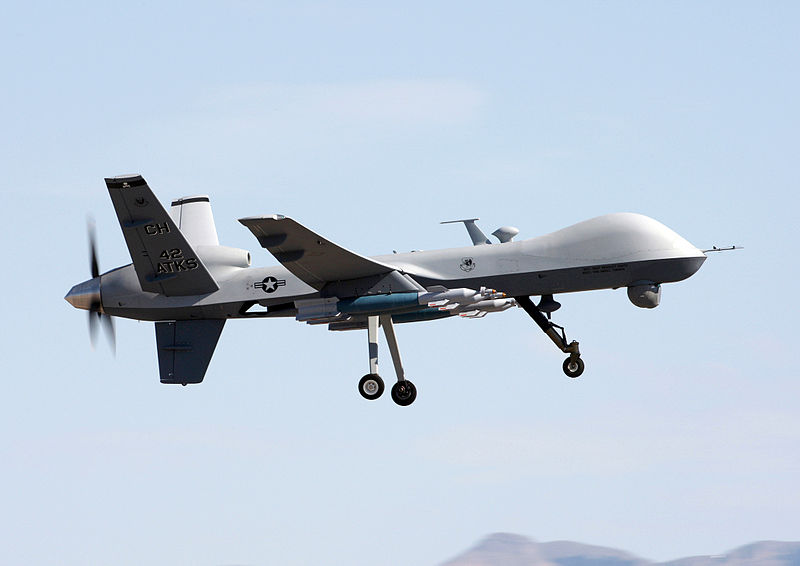
\includegraphics[width=0.48\textwidth]{img/reaper.jpg}
  \end{center}
  \caption{Eine MQ-9 Reaper bei einem Trainingseinsatz.©gemeinfrei}
  \label{reaper}
\end{wrapfigure}

Dies ermöglicht es eine Aufklärungsmission zu erfüllen wie zum Beispiel ein \ac{UAV} über Peking(VR China), gestartet und gesteuert aus Deutschland. Kontrolliert wird der Global Hawk von einem Kontrollzentrum aus, gestützt von modernster Satellitenkommunikation.
Militärische Drohnen können auch Bomben und Raketen aufnehmen. Der erstmalige Einsatz bewaffneter Drohnen ereignete sich am 27. Oktober 2007. Die \ac{MQ-9}(dt.Sensenmann,siehe Abbildung: \ref{reaper}) kann mit zwei 500 Pfund Bomben und vier Hellfire Raketen ausgestattet werden. Sie wurde schon in einigen Einsätzen in Krisengebieten für Luftschläge eingesetzt \cite{MQ-9}.

Zum Anderen werden \acp{UAV} im privaten Sektor für vielfältige Aufgaben eingesetzt. In der Agrarwirtschaft werden sie z.B. zur Detektion von Wildvieh in Anbauflächen eingesetzt (siehe Abbildung \ref{rehkitz}). 
Mittels hochsensiblen Wärmebildkameras kann so ein Zusammenstoß mit Erntemaschinen vermieden werden. Mit diversen Hochleistungskameras und Sensoren kann z.B. der Stickstoffgehalt aus hyperspektralen Bilddaten erkannt werden\cite{workshop_agrar}. Um Pflanzenschutzmittel gezielt in den Bewuchs einzubringen nutzt werden Aufnahmnen von \ac{UAV} genutzt, um Unkrautballungen auf z.B. Ackerflächen zu identifizieren\cite{unkraut}. Selbst das Ausbringen von Pflanzenschutzmitteln auf Ackerland ist mit \ac{UAV} durchaus möglich\cite{holzapfel}.\parfillskip=0pt
 In der Forschung werden \ac{UAV} zur Beobachtung von, für den Menschen unzugänglichen bzw. zu gefährlichen Orten benutzt.\par So kann z.B. radioaktiv verseuchtes Gebiet oder ein aktiver Vulkan untersucht werden ohne das Menschenleben gefährdet werden. Des Weiteren werden sie für Inspektionen an schwer zugänglichen Stellen von Hochspannungsmasten und Brückenpfeilern benutzt. In der Vergangenheit mussten diese Tätigkeiten von einem erfahrenen Helikopterpiloten durchgeführt werden. Diese Arbeiten waren sehr kostenintensiv und gefährlich.


\begin{wrapfigure}{r}{0.6\textwidth}
  \begin{center}
    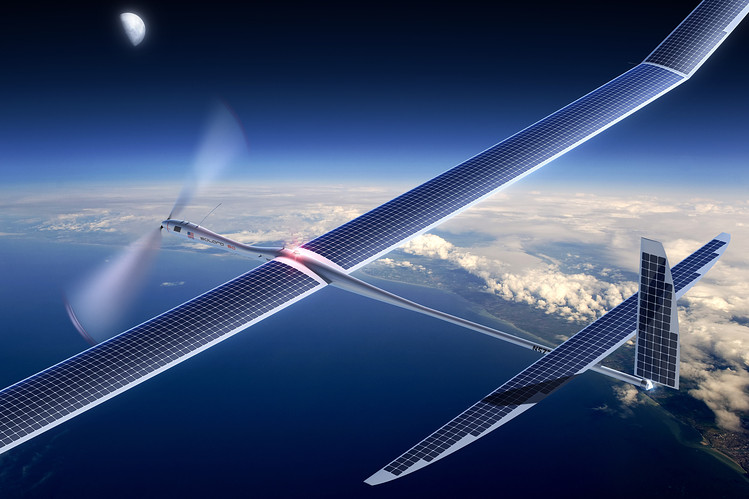
\includegraphics[width=0.5\textwidth]{img/solara50.jpg}
  \end{center}
  \caption{Eine Solara 50.©Titan Aerospace}
  \label{solara}
\end{wrapfigure}

Sie dienen als Relaisstationen für Daten bzw. Kommunikation jeglicher Art. So können \acp{UAV} in großen Höhen Funksignale empfangen und an Empfänger, die durch die Erdkrümmung oder funkstörender Objekte nicht direkt erreicht werden können, weitergeben. Erst kürzlich kaufte der Internetkonzern \textit{Google} den Solardrohnenhersteller \textit{Titan Aerospace}. Die daraus entwickelten Drohnen vom Typ Solara 50 (siehe Abbildung nebenstehend \ref{solara}) sollen eng verbunden mit Googles Projekt Loon als Relaisstationen Internet in die entlegensten Orte auf der Welt bringen. Es soll ein Gürtel aus Solara 50 und gasgefüllten Ballons in einer Höhe von 18 bzw. 32 Kilometern um die Erde gelegt werden. Die Solara 50 kann bis zu 5 Jahre ohne Landung eigenständig in der Luft bleiben \cite{loon}\cite{loon2}.
Wo früher noch aufwendige Luftaufnahmen per Helikopter notwendig waren, werden heute \ac{UAV} mit hochauflösenden Filmkameras ausgerüstet und fliegen äußerst flexibel über Drehsets.
Feuerwehren nutzen die Luftaufklärung zur Ermittlung von Brandherden(siehe dazu:\href{http://youtu.be/_yngOox3oJ4}{Youtube - Luftaufnahme Großbrand}).
Für Städte, Firmen und Tourismusagenturen ist es eine kostengünstige Möglichkeit Luftaufnahmen der Region/ Unternehmung in Imagefilme einzubinden. Auch die Deutsche Telekom nutzt \ac{UAV} um gegen Kupferdiebstahl vorzugehen. Es ist geplant per \ac{UAV} oberirdische Kupferleitungen mit eine Lösung zu bestreichen. Diese Flüssigkeit leuchtet unter \acs{UV-Licht} gelbgrün. Identifiziert wird auf zwei Wegen, zum einen besteht diese künstliche \glqq \acs{DNA}\grqq\ aus verschiedenen Basen. Deren typische Zusammenstellung ermöglicht ein klares zuordnen bei einem Kabeldiebstahl. Der zweite Weg geht über 400 Mikromillimeter kleine Nickelplättchen in der Flüssigkeit. Auf diesen Plättchen sind Identifkationscodes eingraviert die unter einem Mikroskop abgelesen werden können\cite{telekom}.

\newpage
\section{Die DJI Phantom 2 Vision Plus\cite{phantom}}
Die DJI Phantom 2 Vision Plus ist ein Multikopter. Er hat mehrere Rotoren die für den Auftrieb zuständig sind, im Gegensatz zum Helikopter (ein Rotor plus Steuer).
\begin{wrapfigure}{l}{0.6\textwidth}
  \begin{center}
    \includegraphics[width=0.55\textwidth]{img/dji/Dji1.jpg}
  \end{center}
  \label{dji}
  \caption{Eine offene DJI Phantom Vision 2 Plus.©eigenes}
\end{wrapfigure} In diesem Fall handelt es sich um einen Quadrocopter, der von vier Rotoren angetrieben wird. Die vier Rotoren sorgen für den stabilen Flug, sodass keine weiteren Steuertechniken nötig sind. Die Rotoren werden durch bürstenlose Motoren angetrieben (sogenannte \textit{Brushless-Motoren}), die direkt an den vier Armen befestigt sind. So muss die Kraft nicht über Wellen etc. an die Rotorblätter übergeben werden. 
\\
\\
\\
\\
\\
\\
\subsection{Sensoren und Steuergerät}

Damit ein Quadrocopter überhaupt fliegen kann, ist ein Zusammenspiel von diversen Sensoren und Steuergeräten nötig. Im folgenden Abschnitt werden die grundlegenden Bauteile näher beschrieben.\\
\subsubsection*{NAZA-M V2}
Das NAZA-M V2 ist das von DJI entwickelte Steuergerät des Kopters. In ihm laufen alle Sensorwerte und Steuersignale zusammen. Das NAZA-M steuert anhand dieser Messwerte die Drehzahl der vier Rotoren. Desweiteren hat es verschiedene Modi integriert die einen stabilen und sicheren Flug gewährleisten.\\
\subsubsection*{barometrischer Höhensensor}
Der Höhensensor misst anhand des Luftdrucks die derzeitige Höhe. Die Differenz zwischen Luftdruck bei Start und derzeitigem Luftdruck ergibt die Höhe. Diese Methode ist nicht sehr genau, da der Luftdruck Schwankungen unterliegt. In Zusammenspiel mit der Satellitennavigation funktioniert es aber zuverlässig.\\
\subsubsection*{\ac{GPS}}
Ein \ac{GPS} Empfänger erfasst den aktuellen Standort der Phantom 2 Plus. Über ihn ist ein autarker Flug anhand von vorher definierten Wegpunkten möglich. Die Phantom 2 Plus merkt sich den Startpunkt und kann bei ausfallen der Funkverbindung oder anderer Probleme selbständig zu diesem zurückkehren. Anhand des \ac{GPS} ist auch immer eine genaue Ausrichtung zu dem Piloten als Bezugspunkt möglich. Der \ac{GPS}-Empfänger ist direkt unter dem Deckel der Verkleidung angebracht um einen möglichst guten Empfang der \ac{GPS}-Signale zu gewährleisten.
\subsubsection*{Gyroskop}
Über ein Gyroskop, auch Kreiselinstrument genannt, kann die Ausrichtung des Flugobjektes erfasst werden. Der Vorwärtsflug des Phantom 2 Plus wird realisiert, indem die Drehzahl der Rotoren angepasst wird, sodass ein Kippen in Flugrichtung erfolgt. Anhand der Messdaten des Gyroskopes kann die Neigung gesteuert werden. Es wird um maximal 45° nach vorne gekippt, um ein \glqq Überkippen\grqq\ zu verhindern.\\
\subsubsection*{Accelerometer/Beschleunigungssensor}
Beschleunigungssensoren messen den Beschleunigungszuwachs bzw. die Abnahme der Beschleunigung. Zusammen mit dem Gyroskop sorgen sie für ein stabiles Flugbild. Die Bewegungsrichtung und Beschleunigung sind dem Steuergerät somit bekannt\cite{beschleunigung}.
\subsubsection*{Kompass}
Bei \ac{GPS} Navigation kann bei Stillstand/Schwebezustand die Ausrichtung des Objektes nicht genau bestimmt werden. Anhand eines Kompasses kann die Ausrichtung der Phantom 2 Plus auch im Schwebezustand einwandfrei für weitere Funktionen genutzt werden. Der Kompass ist extern an einem Bein des Kopters angebracht um mögliche Interferenzen mit den anderen elektronischen Bauteilen zu verhindern.\\
\subsubsection*{WLAN Sendeeinheit}
Über eine 2,4 GHz WLAN-Verbindung wird das Sucherbild der Kamera übertragen. Da die maximal in Deutschland zulässigen 100 mW nicht überschritten werden dürfen, ist ein Repeater an der Fernbedienung angebracht. Dieser empfängt das Signal und leitet es an ein Smartphone weiter. Das an der Fernbedienung montierte Smartphone liefert welches in der Lage ist das Bild der Kamera live zum fliegen bereitzustellen. Die Flug- und Gerätedaten wie Höhe, Akkuzustand und Speicherstand können über das Smartphone abgefragt werden. Die Ausrichtung der Kamera wird in horizontaler und vertikaler Neigung über den Touchscreen gesteuert. Die Reichweite wird mit ca. 500-700 Metern bei Sichtverbindung angegeben.
\subsubsection*{Funkverbindung}
Die Steuersignale der Funkfernbedienung werden über eine 6 Kanal 5.725-5.85 GHz Verbindung übertragen. Die Reichweite wird mit mindestens 700 Metern angegeben.
\subsubsection*{Kamera}
An einem 3D Gimbal, welcher anhand aller Lagesensoren die Verwacklungen durch den Flug ausgleicht, hängt eine Kamera mit 14 Megapixeln (Auflösung von 4384x3288 Pixel). Videoaufnahmen macht sie mit einer Auflösung von 1080p(1920x1080 Pixel). Das Bild des Suchers wird mit verminderter Auflösung direkt über die Wi-Fi-Verbindung auf das Smartphone des Piloten übertragen. Einstellungen wie Ausrichtung,Auflösung, Belichtung etc. lassen sich direkt über die Wi-Fi-Verbindung ansteuern.\\
\subsection{Flugfunktionen\cite{phantom}}
Es gibt eine Reihe von implementierten Funktionen die einen möglichst unkomplizierten Flug ermöglichen sollen. Im folgenden Abschnitt werden die Wichtigsten näher beschrieben.
\subsubsection*{Home-Lock Modus}
Das Quadcopter merkt sich anhand der GPS-Daten den Startpunkt/Home-Punkt, also den Standpunkt des Piloten. Wird im Flug der Home-Lock Modus gestartet, nimmt der Kopter den Home-Punkt als Bezugspunkt. Wird der Steuerknüppel nach rechts oder links gedrückt, zieht der Kopter einen Kreis mit dem Home-Punkt als Kreismittelpunkt. Wird der linke Steuerknüppel nach vorne bzw. hinten gedrückt, nähert/entfernt sich der Kopter dem Ausgangspunkt, egal in welche Richtung das Fluggerät gerade gedreht ist. Dies ist besonders praktisch wenn der Kopter sich nicht im nahen Sichtfeld befindet. Es ist auf weite Distanz schwer zu erkennen in welche Himmelsrichtung der Kopter ausgerichtet ist. Mithilfe vom Home-Lock Modus kann der Kopter aus jeder Lage wieder zum Piloten zurückgesteuert werden.
\subsubsection*{Course-Lock Modus}
Beim Course Lock wird die Ausrichtung beim Start gemerkt. Wird im Flug in den Course-Lock Modus schaltet, fliegt der Kopter immer mit Bezug auf diese Ausrichtung, unabhängig von der derzeitigen Ausrichtung.\\
\subsubsection*{Coming-Home/Failsafe Funktion}
Wenn der Kopter die Steuerfunkverbindung verliert z.B. durch leere Akkus in der Funkfernbedienung, ein Flug außerhalb des Empfangsbereiches, ein Flug hinter ein funkstörendes Objekt (Baum,Haus etc.) oder einen anderen Defekt, dann schaltet das Steuermodul in den Failsafe-Modus.
Ist die Verbindung verloren, wartet der Kopter schwebend an der derzeitigen Stelle auf neue Signale. Nach 10 Sekunden steigt er auf 20 Meter und steuert anhand der GPS Koordinaten zum Startpunkt zurück und landet.\\

\section{Rechtliche Aspekte\cite{ct}}

Im privaten Umgang mit \ac{UAV} sollte sich die Frage gestellt werden: Was ist rechtlich erlaubt und was muss beachtet werden? Die Nutzung von Fluggeräten jeglicher Art ist im \ac{LuftVG}\cite{luftvg} und der \ac{LuftVO}\cite{luftvo} geregelt. Dazu werden im nächsten Abschnitt einige wichtige Punkte zusammengefasst.

\subsection{Genehmigungspflicht und generelle Flugverbote}
Für den rein privaten Gebrauch wird keine Aufstiegsgenehmigung vorausgesetzt, sofern das \ac{UAV} nicht über 5 kg Startgewicht hat. Wenn der Einsatz eines \ac{UAV} einen kommerziellen, gewerblichen Grund hat, bedarf es einer Genehmigung seitens des Gesetzgebers. Flugplätze sind von Überflügen ausgeschlossen. In einigen Bundesländern gibt es zudem ausgewiesene Flugverbotszonen
(Regierungsviertel, Atomkraftwerke, Menschenansammlungen und andere).
\subsection{Einschränkungen der örtlichen und personellen Nutzung}
Das \ac{UAV} sollte in Sichtweite des Piloten gesteuert werden(200- 300m). Die Flughöhe sollte, je nach Bundesland, 30 bis 100 Meter nicht überschreiten. Grundstücke dürfen nur mit Erlaubnis überflogen werden. Gerade bei niedrigen Überflügen mit Kameravorrichtung stellt es einen Eingriff in die Privatsphäre dar. Bei der Steuerung von privaten, nicht genehmigungspflichtigen \ac{UAV} gilt keine Altersbeschränkung.
\subsection{Haftung}
Der Führer des \ac{UAV} haftet für Schäden, die durch den Flug entstehen. Haftpflichtversicherungen schließen solche Schäden aus. Es gibt spezielle Versicherungsangebote für den Betrieb von \ac{UAV}. Diese sind auch Voraussetzung für eine Aufstiegsgenehmigung.
\subsection{Nutzung des Bildmaterials}
Ein äußerst wichtiger Punkt ist die Regelung zur Nutzung von Kamerafunktionen. Bildaufnahmen von Personen sind sehr streng geregelt. So ist es in vielen Fällen notwendig sich Genehmigungen von den jeweiligen Personen, Grundstückeigentümern oder Veranstaltern einzuholen. Bilder auf denen Personen explizit zu erkennen sind bedürfen immer das Einverständnis der Personen, da sonst das Recht am eigenen Bild verletzt wird. Ausnahme sind dabei öffentliche Veranstaltungen, wenn die betreffenden Personen nicht das Hauptmotiv des Bildes sind, sondern die Veranstaltung an sich. Motive von Gebäuden dürfen, solange sie die öffentlich zugängliche Seite belichtet, in privatem Umfeld gezeigt werden. Sollten die Bilder veröffentlicht werden, so unterliegen Luftaufnahmen nicht der Panoramafreiheit\cite{Panoramafreiheit}. Das bedeutet es dürfen nur Bilder, die von öffentlichen Orten ohne Zuhilfenahme von Hilfsmitteln (Hubschrauber, \ac{UAV}, Leitern) gemacht werden, genutzt und veröffentlicht werden. Militärisch genutzte Bereiche und Geräte dürfen nicht aufgenommen werden, sobald es zu Nachteilen für die Sicherheit der Bundesrepublik Deutschland kommen kann.

\input{06_Fazit/Fazit}

\newpage
%\section*{Abkürzungsverzeichnis}
\addsec{Abkürzungsverzeichnis}

\begin{acronym}[UV-Licht]
\acro{UAV}{Unmanned aerial vehicle}
\acro{V2}{Vergeltungswaffe 2}
\acro{RP-1}{Radio Plane 1}
\acro{MQ-9}{General Atomics MQ-9}
\acro{GPS}{Global Positioning System}
\acro{LuftVG}{Luftverkehrsgesetz}
\acro{LuftVO}{Luftverkehrsordnung}
\acro{UV-Licht}{ultraviolettes Licht}
\acro{DNA}{deoxyribonucleic acid}
\end{acronym}



\bibliography{literatur}
\newpage




\begin{figure}[p]
\begin{center}
\addsec{Anhang - Abbildungen}
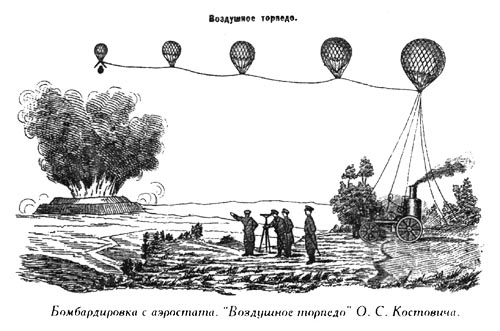
\includegraphics[scale=0.5]{img/balloonbombs.jpg}
\caption{Luftangriff per Ballon,©Prof. Jurij Drushnin, Moscow, Russia}
\label{ballonbombs}
\end{center}
\end{figure}

\begin{figure}[p]
\begin{center}
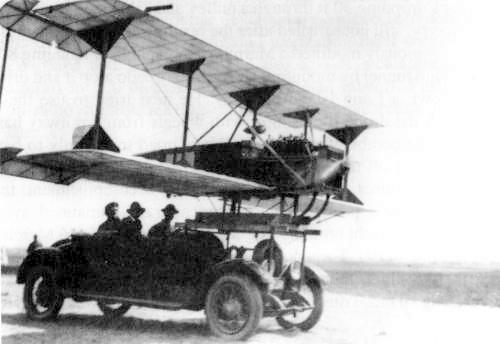
\includegraphics[scale=0.5]{img/flying_bomb.jpg}
\caption{Hewitt-Sperry Automatic Airplane,©uavglobal.com}
\label{Flying Bomb}
\end{center}
\end{figure}

\begin{figure}[p]
\begin{center}
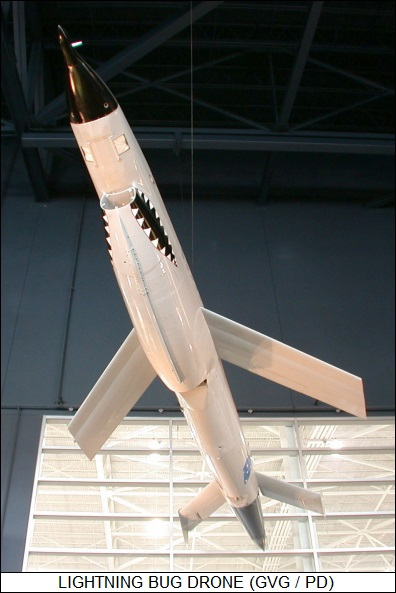
\includegraphics[scale=0.5]{img/fire_fly.jpg}
\caption{Ryan Model 147A (Fire Fly),©creativecommons}
\label{fire fly}
\end{center}
\end{figure}

\begin{figure}[p]
\begin{small}
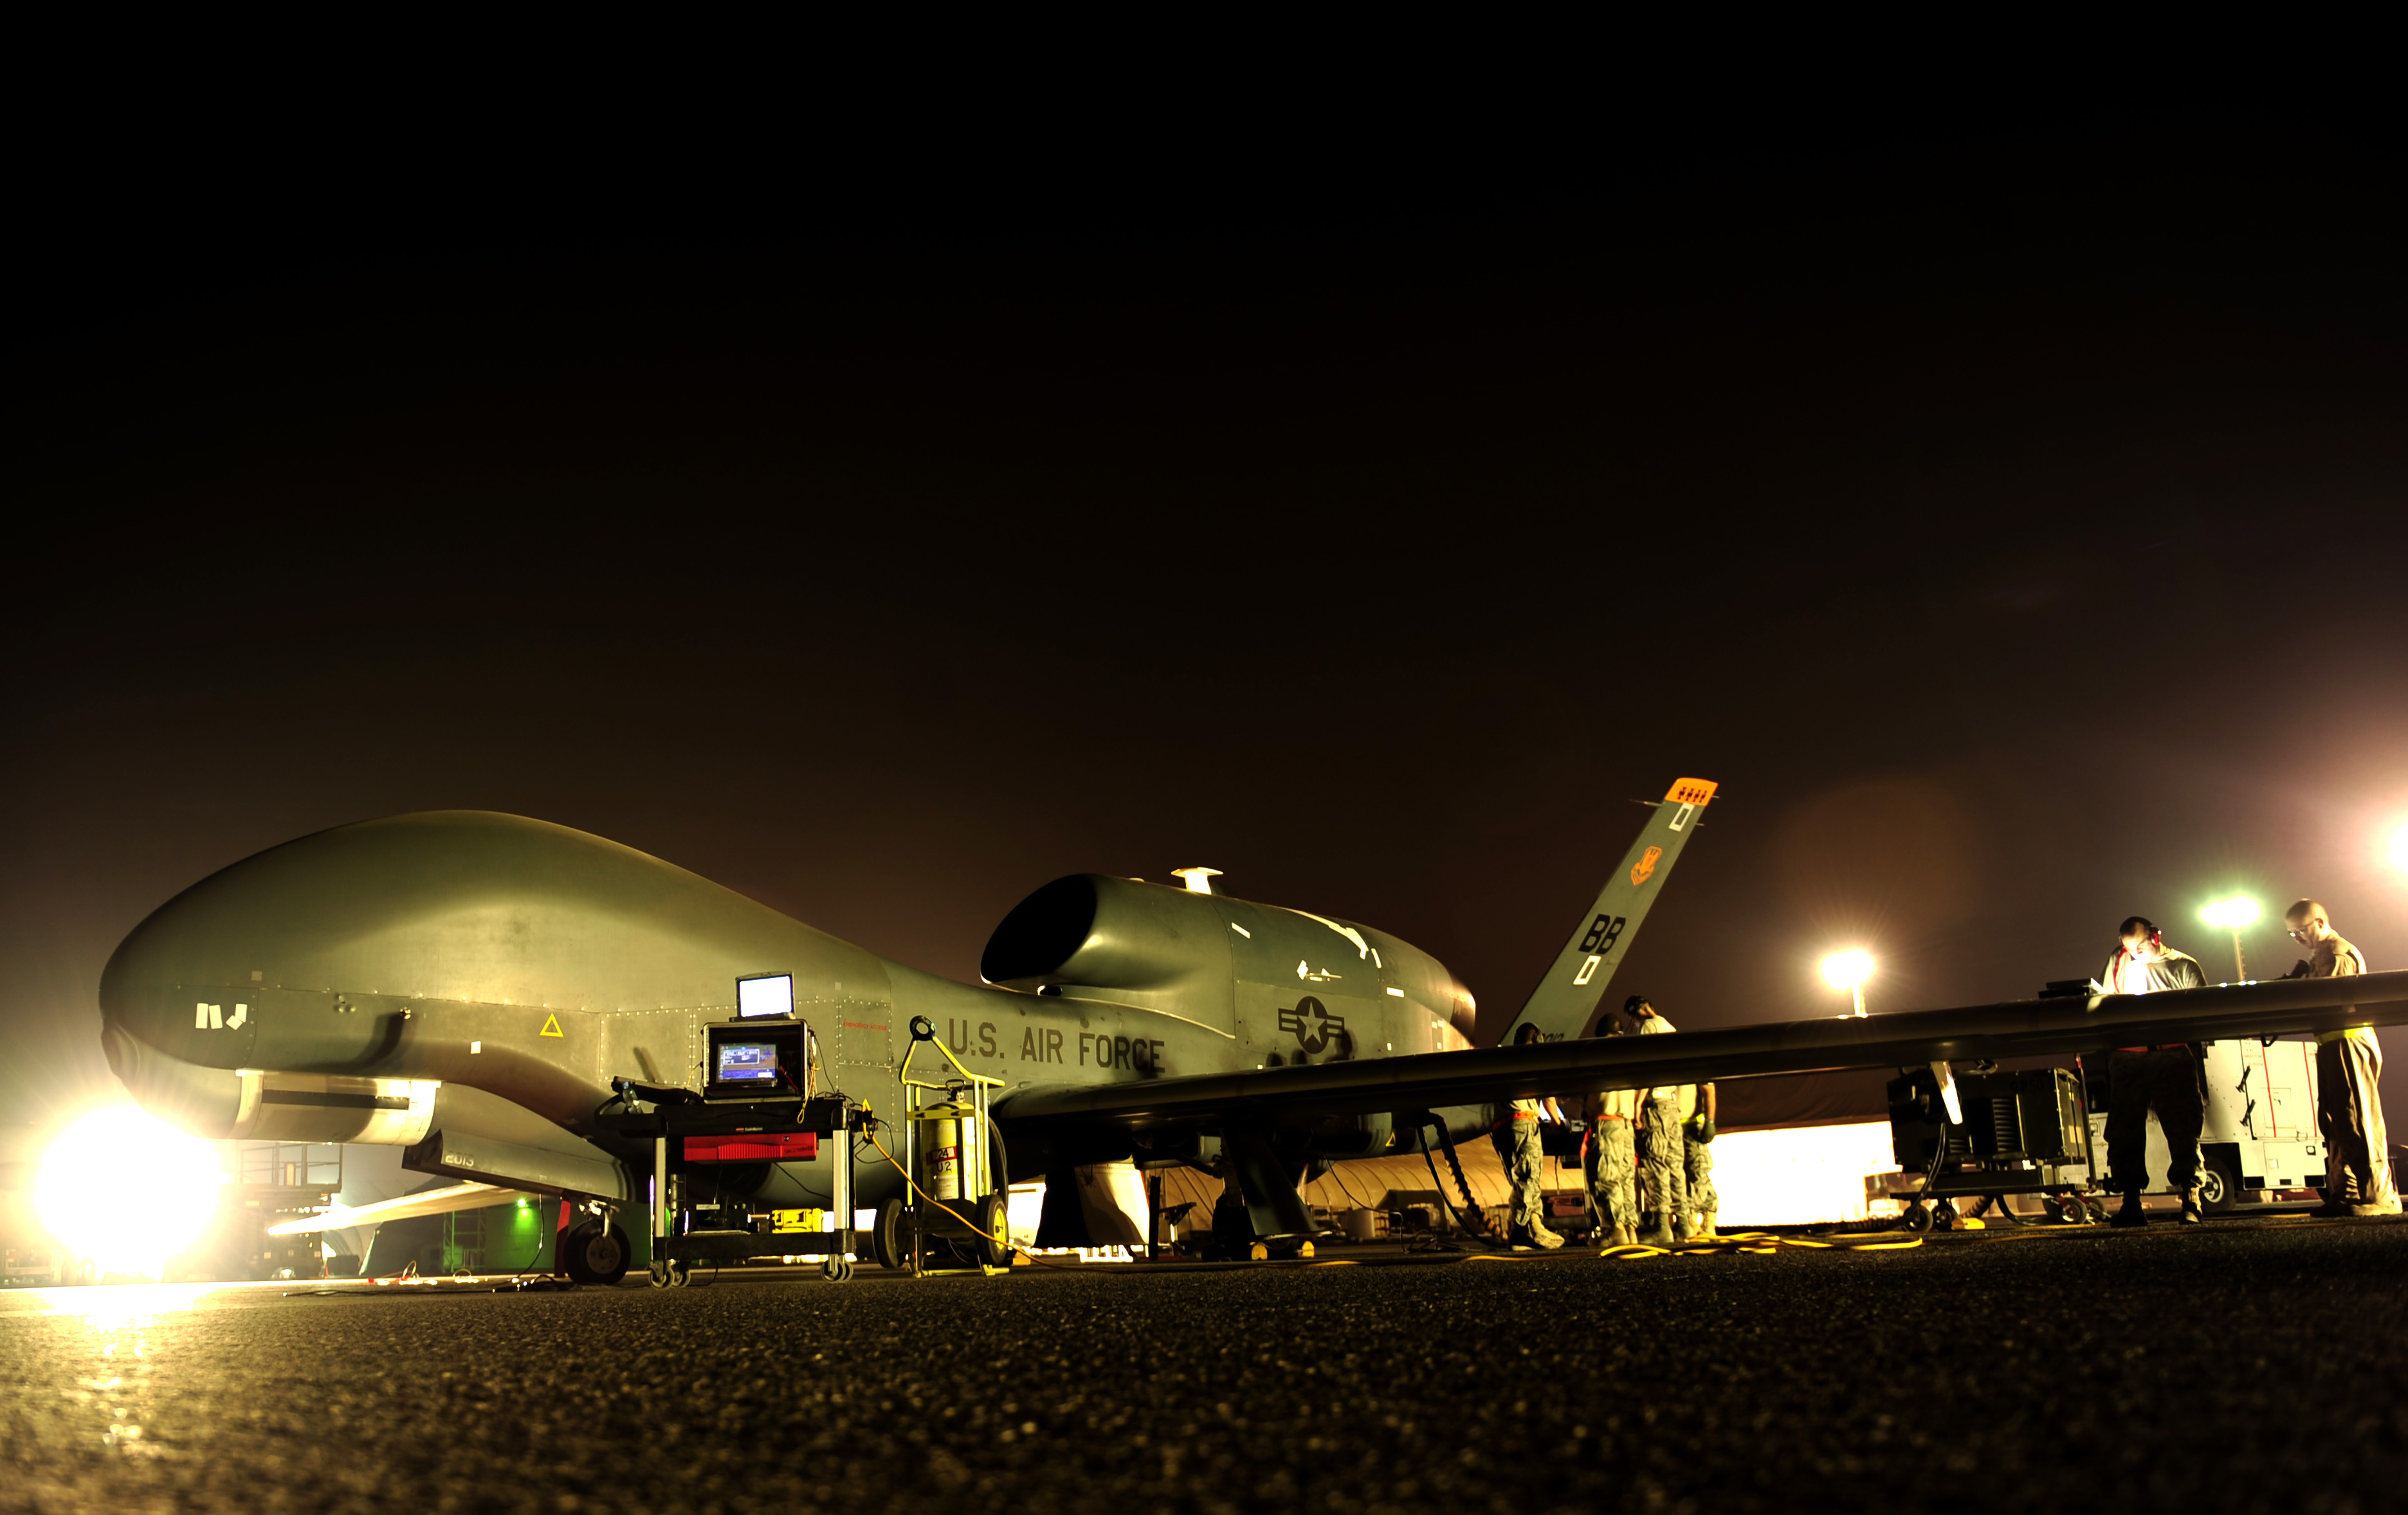
\includegraphics[scale=0.4]{img/rq-4b.jpg}
\caption{Northrop Grumman RQ-4 (Global Hawk),©af.mil,frei}
\label{global hawk}
\end{small}
\end{figure}

\begin{figure}[p]
\begin{small}
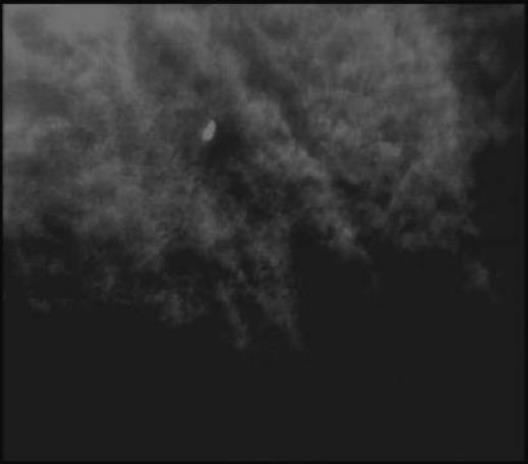
\includegraphics[scale=0.8]{img/Rehkitz.jpg}
\caption{Thermalbild eines Rehkitzes in einem Kornfeld aus 50m Höhe,©Leibniz-Institut für Agrartechnik}
\label{rehkitz}
\end{small}
\end{figure}

%\begin{figure}[p]
%\begin{small}
%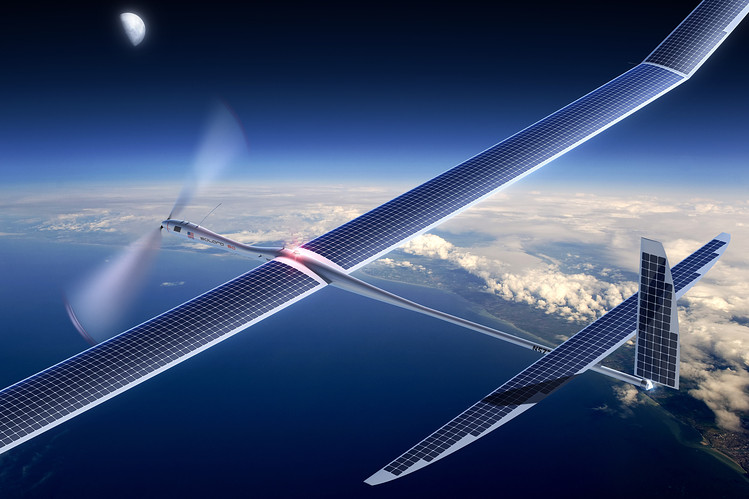
\includegraphics[scale=0.5]{img/solara50.jpg}
%\caption{Solara 50 von Titan Aerospae,©Titan Aerospace}
%\label{solara}
%\end{small}
%\end{figure}


\end{document}



